%%%%%%%%%%%%%%%%%%%%%%%%%%%%%%%%%%%%%%%%%
% Medium Length Professional CV
% LaTeX Template
% Version 2.0 (8/5/13)
%
% This template has been downloaded from:
% http://www.LaTeXTemplates.com
%
% Original author:
% Trey Hunner (http://www.treyhunner.com/)
%
% Important note:
% This template requires the resume.cls file to be in the same directory as the
% .tex file. The resume.cls file provides the resume style used for structuring the
% document.
%
%%%%%%%%%%%%%%%%%%%%%%%%%%%%%%%%%%%%%%%%%

%----------------------------------------------------------------------------------------
%	PACKAGES AND OTHER DOCUMENT CONFIGURATIONS
%----------------------------------------------------------------------------------------

\documentclass{resume} % Use the custom resume.cls style

\usepackage{hyperref}
\usepackage{graphicx}
\usepackage{fontawesome5}
\usepackage[usenames,dvipsnames]{xcolor}
\usepackage[left=0.5in,top=0.6in,right=0.5in,bottom=0.6in]{geometry} % Document margins
%\newcommand{\tab}[1]{\hspace{.2667\textwidth}\rlap{#1}}
%\newcommand{\itab}[1]{\hspace{0em}\rlap{#1}}

% \address{ +98 933 5098928 }
% \address{\url{https://hamidrezakmk.github.io/}} % Your Personal webpage
% %\address{123 Pleasant Lane \\ City, State 12345} % Your secondary addess (optional)
% \address{ hamidrezakamkari@gmail.com }
% \name{Hamidreza Kamkari} % Your name


\begin{document}
\begin{minipage}{0.48\textwidth}
{\Huge \textcolor{RoyalPurple!100}{\bf Hamidreza} \textcolor{RoyalPurple!100}{\scshape \bf Kamkari}}\\
\\
‌\hspace{6mm} \faAt \ \ \textcolor{Black!70}{\href{mailto:hamidrezakamkari@gmail.com}{hamidrezakamkari@gmail.com}}\\
‌\hspace{6mm} \faGlobe \ \ \textcolor{Black!70}{\href{https://hamidrezakmk.github.io/}{\underline{HamidrezaKmK.github.io}}}\\
‌\hspace{6mm} \faPhone \ \ \textcolor{Black!70}{+98 933 5098928}\\
\end{minipage} \begin{minipage}{0.48\textwidth}
\begin{flushright}
\fcolorbox{RoyalPurple}{CadetBlue}{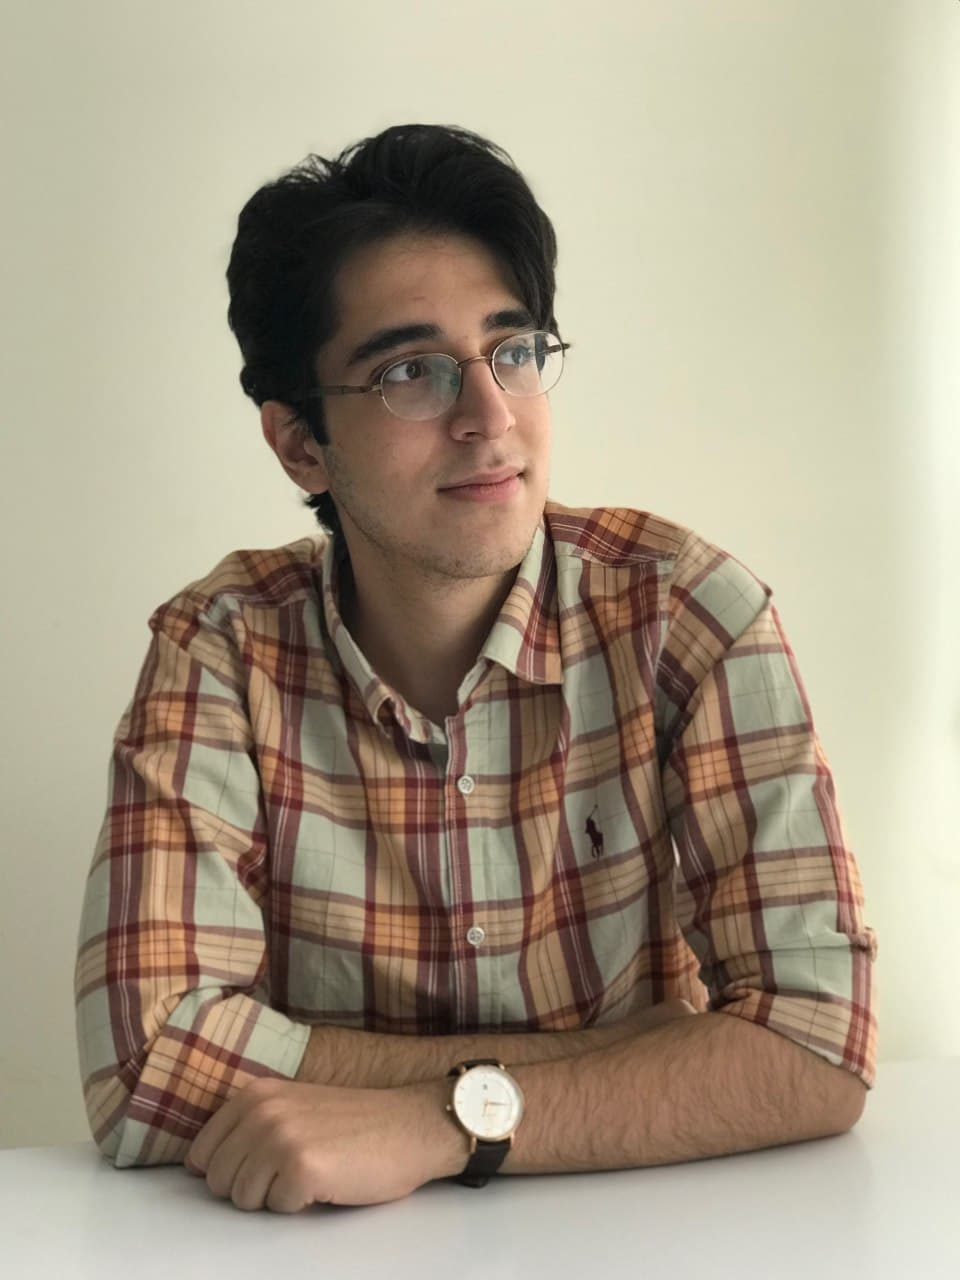
\includegraphics[width=7em]{me.jpg}}
\end{flushright}
\end{minipage}
\\
%----------------------------------------------------------------------------------------
%	EDUCATION SECTION
%----------------------------------------------------------------------------------------

\begin{rSection}{Education}

{\bf Sharif University of Technology} \hfill \textcolor{Black!70}{\em 2018 - 2022} 
\\ Bachelor of Science \hfill \textcolor{Black!70}{ Overall GPA 19.38/20 | Last Year GPA 19.93/20}
\\ Department of Computer Engineering \hfill \textcolor{Black!70}{Ranked Among the Top 6\%}
\\
\\{\bf AE Highschool} \hfill \textcolor{Black!70}{\em 2016 - 2018} 
\\ Higher Secondary Education \hfill \textcolor{Black!70}{ Overall Score 19.23/20}
\\ Mathematics, Physics
\\
% \\{\bf Qazvin's School for Exceptional Talents (\href{https://en.wikipedia.org/wiki/National_Organization_for_Development_of_Exceptional_Talents}{\underline{NODET}})} \hfill \textcolor{Black!70}{\em2011 - 2016}
% \\ Secondary Education \hfill \textcolor{Black!70}{Overall Score 20/20}
% \\ State Board \hfill \textcolor{Black!70}{ State Rank-1}



\end{rSection}
%----------------------------------------------------------------------------------------
%	WORK EXPERIENCE SECTION
%----------------------------------------------------------------------------------------

\begin{rSection}{Research and Publication}


\begin{rSubsection}{Sharif University of Technology}{\textcolor{Black!70}{\bf Tehran, Iran}}
{Predicting Drug Combination Effects by Utilizing Chemical \& Multi-Omics Data}{\textcolor{Black!70}{January 2022 - Ongoing}}
\item {\tt (Preparing manuscript for submission)}
\begin{small}
\item We used Graph Neural Networks and Attention mechanisms to create a general state-of-the-art framework for predicting drug dose response using SMILES representation of drugs.
\end{small}
\end{rSubsection}

%------------------------------------------------

\begin{rSubsection}{Maxplanck Institute of Informatics (MPI-INF)}{\textcolor{Black!70}{\bf Saarbrücken, Germany}}
{Designing nature-based algorithm to solve Semi-Definite Programs (SDP)}
{\textcolor{Black!70}{August 2020 - July 2022}}
\item {\tt(Submitted to SODA) arXiv:2111.02291 [cs.ds, math.co]} \begin{small}
\item We produced a general recipe to create algorithms to address SDPs based on previous work on nature-inspired LP dynamics. We have provided proof and empirical results in our paper to back up our findings.
\end{small}
\end{rSubsection}
\begin{rSubsection}{Maxplanck Institute of Informatics (MPI-INF)}{\textcolor{Black!70}{\bf Saarbrücken, Germany}}
{Fine-Grained Complexity of Optimizing Bias Terms on Neural Networks}
{\textcolor{Black!70}{January 2022 - February 2022}}
\begin{small}
\item Under the supervision of Andreas Karrenbauer and with the collaboration of Karl Bringmann, we devised tight bounds for the complexity of fine-tuning bias terms of neural networks.
\end{small}
\end{rSubsection}

\begin{rSubsection}{Aalto University}{\textcolor{Black!70}{\bf Finland}}
{RNA sequence design using Graph Neural Networks}
{\textcolor{Black!70}{July 2021 - September 2021}}{}
\begin{small}
\item We created a data-driven black box approach for RNA sequence design. The topic involved a baseline familiarity with RNA structures and an in-depth understanding of Graph Neural Network architectures and machine learning basics.
\end{small}
\end{rSubsection}

\end{rSection}


%	EXAMPLE SECTION
%----------------------------------------------------------------------------------------

%----------------------------------------------------------------------------------------
%	TECHNICAL STRENGTHS SECTION
%----------------------------------------------------------------------------------------

\begin{rSection}{Academic Experience}
\begin{rSubsection}{Teaching Assistance}{\textcolor{Black!70}{\bf Sharif University of Technology, Iran}}{}{}
\begin{small}
\item Artificial Intelligence course (CE40417) \href{http://blogs.bu.edu/mhrohban/}{\underline{Mohammad Hossein Rohban}} \hfill \textcolor{Black!70}{\it September 2021 - January 2022}
\item {\bf Head}  of Data Structure and Algorithms course (CE40254) - \href{http://sharif.edu/~ghodsi/}{\underline{Mohammad Ghodsi}} \hfill \textcolor{Black!70}{\it January 2021 - June 2021}
\item Artificial Intelligence course (CE40417) \href{http://blogs.bu.edu/mhrohban/}{\underline{Mohammad Hossein Rohban}} \hfill \textcolor{Black!70}{\it January 2021 - June 2021}
\item Probability and Statistics course (CE40181) \href{https://scholar.google.com/citations?user=GbJMZLIAAAAJ&hl=en}{\underline{Ali Sharifi-Zarchi}} \hfill \textcolor{Black!70}{\it September 2020 - January 2021}
\item Discrete Structures course (CE40115) \href{https://scholar.google.com/citations?user=xuNJ-d8AAAAJ&hl=en}{\underline{Mohammad Ali Abam}} \hfill \textcolor{Black!70}{\it January 2020 - June 2020}
\item Advanced Algorithm design course (CE40354) \href{https://scholar.google.com/citations?user=GbJMZLIAAAAJ&hl=en}{\underline{Ali Sharifi-Zarchi}} \hfill \textcolor{Black!70}{\it January 2020 - June 2020} 
\item Data structure and Algorithms course (CE40254) \href{https://scholar.google.com/citations?user=TNfL9SIAAAAJ&hl=en}{\underline{Mahdi Safarnejad-Boroujeni}} \hfill \textcolor{Black!70}{\it January 2020 - June 2020}
\item Data structure and Algorithms course (CE40254) \href{https://scholar.google.com/citations?user=TNfL9SIAAAAJ&hl=en}{\underline{Mahdi Safarnejad-Boroujeni}} \hfill \textcolor{Black!70}{\it September 2019 - January 2020}
\end{small}
\end{rSubsection}
\end{rSection}

\begin{rSection}{Work Experience}
\begin{small}
\begin{rSubsection}{Fanap IT Company}{\textcolor{Black!70}{\it January 2022 - Present}}{}{}
\itemsep -2pt
\item Our work at Fanap involves dealing with an object detection model able to analyze OPG (Orthopantomogram) images and detect certain tooth features automatically. This project facilitates machine learning and computer vision techniques in the context of medical image processing.
\end{rSubsection}
\begin{rSubsection}{National Olympiad in Informatics Committee}{\textcolor{Black!70}{\it September 2020 - December 2021}}{}{}
\itemsep -2pt
\item My work involves careful curating of national competitive contests for talented nationwide students as well as coordinating educational programs related to computer science and algorithms. As a member, I have created a graph theory course and organized the Iranian IOI team selection contests.
\end{rSubsection}
\begin{rSubsection}{Mentor-ship, Teaching, and Online Educational Content}{}{}{}
\itemsep -1pt
\item \parbox{15cm}{Teaching creative algorithm design as well as basics of data science to employees of computer science-related companies in MAPSA boot camp.} \hfill
\parbox{3cm}{\begin{flushright}
\begin{center}
\textcolor{Black!70}{\it June 2020 \\ August 2020}
\end{center}
\end{flushright}}
\item \parbox{15cm}{Computer Olympiad Teacher in well-known Iranian high schools as well as a mentor at IOI preparation camp for \href{https://ioi2019.az/}{International Olympiad in Informatics held in Baku, Azarbaijan}.} \hfill 
\parbox{3cm}{\begin{flushright}
\begin{center}
\textcolor{Black!70}{\it January 2019 \\ February 2019}
\end{center}
\end{flushright}}
\item \parbox{15cm}{Leader of Quera College content creation team in {\it Quera} IT company. My work involved creating online courses that focus on the basics of programming as well as creative algorithm design. I and my colleagues created two online courses on {\it Basics of Programming} and {\it Advanced Design of Algorithms and Data-structures} that were used nation-wide with almost 4000 participants.} \hfill 
\parbox{3cm}{\begin{flushright}
\begin{center}
\textcolor{Black!70}{\it June 2018 \\ July 2019}
\end{center}
\end{flushright}}
\end{rSubsection}
\end{small}
\end{rSection}

\begin{rSection}{Honors and Awards}
\begin{footnotesize}
\begin{minipage}[t]{1.6in}
\begin{center}
\vspace{0.2cm}
    \faLink \ \href{http://icpc.sharif.edu/2018/scoreboard/}{\bf \underline{ACM-ICPC}}\\
    Regional Gold Medal\\
    Team ranked 3rd\\
    \textcolor{Black!70}{\it December 2018}
\end{center}
\end{minipage}
\hspace{0.1cm}
\begin{minipage}[t]{1.6in}
\begin{center}
\vspace{0.2cm}
\faLink \ \href{https://apio2018.ru/results/official-contest/}{\bf \underline{APIO}}\\
Asia-Pacific Informatics\\
Bronze Medal \\
\textcolor{Black!70}{\it May 2018}
\end{center}
\end{minipage}
\hspace{0.1cm}
\begin{minipage}[t]{1.6in}
\begin{center}
\vspace{0.2cm}
\faLink \ \href{https://www.info1cup.com/archive/2018/International_Round_Ranking.pdf}{\bf \underline{INFO-Cup}} \\
World-wide contests\\
Gold Medal\\
\textcolor{Black!70}{\it March 2018}
\end{center}
\end{minipage}
\hspace{0.1cm}
\begin{minipage}[t]{1.8in}
\begin{center}
\vspace{0.2cm}
\faLink \ {\bf \href{https://ioinformatics.org/journal/v11si_2017_25_33.pdf}{\underline{Olympiad in Informatics}}} \\
Gold and Silver Medal\\
In National Contests\\
\textcolor{Black!70}{\it September of 2016 \& 2017}
\end{center}
\end{minipage}
\end{footnotesize}
\end{rSection}
%----------------------------------------------------------------------------------------
\begin{rSection}{Relevant Courses}
{\bf Core Courses} \hfill \textcolor{Black!70}{\bf Sharif University of Technology}
\vspace{0.15cm}
\begin{small}
\\ ‌\hspace{0.7cm} \parbox{17cm}{Statistics and Probabilities (20/20), Technical Presentation (20/20), Artificial Intelligence (20/20), Algorithm Design (20/20), Algorithms and Data-Structures (20/20), Bio-Informatics (20/20), Modern Information Retrieval (20/20), Stochastic Processes (Graduate Course - 19.8/20), Linear Algebra (20/20), Numerical Computation (20/20), Signals \& Systems (20/20), Operating Systems (20/20), Computer Networks (18.8/20)}
\end{small}
\\ {\bf Online Courses}
\begin{small}
\\ ‌\hspace{0.7cm} Introduction to Machine learning, Coursera online course by Andrew Ng, HSE Advanced Machine Learning Coursera
\end{small}
\end{rSection}

\begin{rSection}{SKILLS}
\begin{minipage}[t]{3.2in}
\begin{center}
{\bf Programming Skills:} 

\begin{footnotesize} Python, Pytorch, Sklearn, Docker, C++ (for competetive programming), Java, MATLAB, \LaTeX. \end{footnotesize}
\end{center}
\end{minipage}
\hspace{0cm}
\begin{minipage}[t]{4in}
\begin{center}
{\bf Languages:}\\
\vspace{0.2cm}
\begin{footnotesize} Persian (Native) - English (Fluent) TOEFL iBT 116/120\\ Speaking: 28/30 - Writing: 29/30 - Reading: 30/30 - Listening: 29/30 
\end{footnotesize}
\end{center}
\end{minipage}
\end{rSection}

%----------------------------------------------------------------------------------------
\begin{rSection}{Technical Projects}
\begin{footnotesize}
\begin{minipage}[t]{1.8in}
\begin{center}
\vspace{0.1cm}
    \faGithub \ \href{https://github.com/HamidrezaKmK/ML-Mnemonist}{\bf \underline{ML-Mnemonist}}\\
    Lightweight Python framework\\
    for ML development\\
    \textcolor{Black!70}{\it Python}
\end{center}
\end{minipage}
\hspace{0.1cm}
\begin{minipage}[t]{1.6in}
\begin{center}
\vspace{0.1cm}
\faGithub \ \href{https://github.com/SharifAIChallenge/AIC20-Client-Python}{\bf \underline{Client AI-challenge}}
Python Client for a game\\
in Sharif AI challenge\\
\textcolor{Black!70}{\it Python}
\end{center}
\end{minipage}
\hspace{0.1cm}
\begin{minipage}[t]{1.6in}
\begin{center}
\vspace{0.1cm}
\faGithub \ \href{https://github.com/HamidrezaKmK/SimpleCServer/}{\bf \underline{Simple C Server}} \\
Server programmed in C\\ 
with multiprocess and multithread capabilities\\
\textcolor{Black!70}{\it C/C++}
\end{center}
\end{minipage}
\hspace{0.1cm}
\begin{minipage}[t]{1.6in}
\begin{center}
\vspace{0.1cm}
    \faGithub \ \href{https://github.com/MostafaOjaghi/DecafCompiler}{\bf \underline{Compiler Design}}\\
    Compiler for object-oriented \\
    programming language\\
    \textcolor{Black!70}{\it C++}
\end{center}
\end{minipage}
\end{footnotesize}
\end{rSection}
%----------------------------------------------------------------------------------------
%----------------------------------------------------------------------------------------

%\begin{rSection}{Miscellaneous} 
% I love traveling, watching movies and TV series. I also appreciate music and into composing in genres of rock and metal. 
 % \item Member, Athletics Team, IIT Kanpur. Attended Summer Sport Camp as a long jumper.
%\item Trained and disciplined in National Cadet Corps (NCC), IIT Kanpur for a year.
 %\item  Participated in Vijyoshi Camp 2012 organized at Indian Institute of Science, Bangalore.
 %\item Won 2nd position in Kho-Kho in Intramurals conducted by Physical Education Section, IIT Kanpur.
 %\item Pursued French as a second language during secondary school from Grade 6 to Grade 10. Also participated in French Song Competition and French G.K. Quiz in Class 10th. %

%\end{rSection}

\end{document}


